\documentclass[12pt, a4paper]{article}

\usepackage[english]{babel}
\usepackage[utf8x]{inputenc}
\usepackage[T1]{fontenc}

\usepackage{apacite}
\usepackage[authoryear]{natbib}
\renewcommand*{\bibfont}{\small}
\renewcommand{\bibsection}{}

\usepackage{amssymb}
\usepackage{amsmath}
\usepackage{fourier}
\usepackage{microtype}
\usepackage{multicol}
\usepackage{graphicx}
\usepackage[top=0.55in,left=0.50in,right=0.50in,bottom=0.55in]{geometry}

% undo the change to mathcal from fourier package
\DeclareMathAlphabet{\mathcal}{OMS}{cmsy}{m}{n}

\usepackage{tikz}
\usetikzlibrary{fit,shapes,arrows,positioning}

\tikzstyle{block} = [draw, rectangle, minimum height=3em, minimum width=3em]
\tikzstyle{ensemble} = [draw, circle, node distance=1cm]
\tikzstyle{input} = []
\tikzstyle{output} = []

\renewcommand{\vec}{\mathbf}  % Bold vectors
\newcommand{\transpose}[1]{{#1}^\mathsf{T}}

\title{Recurrently compressing a rolling time window %into a polynomial state-space
using spiking neurons}
\author{Aaron R. Voelker and Chris Eliasmith}
\makeatletter
\newcommand{\thetitle}{\@title}
\newcommand{\theauthor}{\@author}
\newcommand{\theaffiliation}{
	Centre for Theoretical Neuroscience, University of Waterloo\\
	\{arvoelke, celiasmith\}@uwaterloo.ca}
\makeatother

\begin{document}

{\centering
 \Large\thetitle\\[0.25cm]
 \large\theauthor\\[0.25cm]
 \normalsize\theaffiliation\\[0.5cm]}

\noindent
\textsc{Abstract:} We present a dynamical system that optimally compresses a rolling time window of input into a low-dimensional state-space.
The state of this system represents the history of its input by a linear combination of time-invariant polynomial basis functions.
We use the Neural Engineering Framework~(NEF) to compile this system onto a recurrent spiking neural network.
The activity of this ``delay network'' naturally approximates a Taylor series expansion, over time, centered about every point within the window.
We show that this permits the computation of arbitrary nonlinear computations across the history of an input stimulus, while outperforming Echo State Networks in accuracy and training/testing time, without explicitly simulating any training examples. \\

\noindent
\textsc{Additional Detail:} A continuous-time rolling window of length $\theta > 0$, denoted $[ u(t - \theta') \,:\, 0 \le \theta' \le \theta ]$, may be \emph{temporally compressed} into a low-dimensional state $\vec{x}(t) \in \mathbb{R}^d$, by the following linear time-invariant dynamical system that approximately delays an input signal by $\theta$ seconds~\citep{voelkerdelay2017}:
\begin{equation} \label{eq:delay-system}
  \dot{\vec{x}}(t) = A\vec{x}(t) + Bu(t) \text{,} \quad
  A = \begin{pmatrix} -v_0 & -v_0 & \cdots & -v_0 \\ v_1 & 0 & \cdots & 0 \\ 0 & \ddots & \ddots & \vdots \\ 0 & 0 & v_{d-1} & 0\end{pmatrix} \text{,} \quad 
  B = \transpose{\begin{pmatrix} v_0 & 0 & \cdots & 0\end{pmatrix}} \text{,} 
\end{equation}
where $v_i := \frac{(d+i)(d-i)}{i+1} \theta^{-1}$, %and $w_i := (-1)^{d - 1 - i} \left( \frac{i+1}{d} \right)$
for $i = 0 \ldots d-1$.
%We may also solve this system to express $\vec{x}(t)$ as a convolution of $u$ with the SIMO impulse response $\vec{f}$: 
%\begin{equation} \label{eq:lti-solved}
%\vec{f}(t) = e^{At} B \text{,} \quad \vec{x}(t) = \left(u \ast \vec{f}\right)(t) \text{.}
%\end{equation}
This compression is derived by applying Pad\'e approximants to $e^{-\theta s}$ about the complex point $s=0$, which yields an optimal low-degree polynomial expansion of $\mathcal{L}\{u\}(s)$ about its zeroth frequency.
%\footnote{Note that a LTI system is equivalent up to any invertible linear transformation applied to the state-space.}
The state $\vec{x}(t)$ represents the rolling window via a linear combination of time-invariant polynomial basis functions:
\begin{equation} \label{eq:basis-interpretation}
\boxed{u(t - \theta') \approx \sum_{i=0}^{d-1} \mathcal{P}_{i,d} \left(\frac{\theta'}{\theta} \right) \, x_{d-1-i}(t) \text{,} \quad 0 \le \theta' \le \theta \text{,}}
\end{equation}
which we have solved in closed-form~\citep[][eq.~14]{voelkerdelay2017}:
\begin{equation} \label{eq:basis-functions}
\mathcal{P}_{i,d}(r) = \begin{pmatrix}d \\ i\end{pmatrix}^{-1} \sum_{j=0}^i \begin{pmatrix}d \\ j\end{pmatrix} \begin{pmatrix}2d - 1 - j \\ i - j\end{pmatrix} \left( -r \right)^{i - j} \text{.} %\text{,}\quad 0 \le r \le 1 \text{,}\quad i = 0 \ldots d - 1
\end{equation}
A set of polynomials $\{ \mathcal{P}_{i, d} \}$ are shown in Figure~\ref{fig:basis}.
This defines a linear map from the $d$-dimensional state, $\vec{x}(t)$, to the infinite-dimensional rolling window, $[ u(t - \theta') \,:\, 0 \le \theta' \le \theta ]$.
In other words, (\ref{eq:basis-interpretation}) is the optimal pseudoinverse of the linear compression defined by (\ref{eq:delay-system}).
%The frequencies in $u(t)$ that may be accurately encoded by this approach scale inversely with $\theta$.
%Likewise, higher values of $q$ allowed for higher frequencies to be encoded at the same level of precision.
%We remark that each basis function is expressed in terms of the unitless quantity $\frac{\theta'}{\theta}$, and is therefore scale-invariant.
%We may also transform the state by any invertible matrix (e.g.,~ to orthogonalize the basis functions) without loss of generality.
%Analysis of the approximation error, and some additional properties of this ``delay network'', may be found in \cite{voelkerdelay2017}.
Moreover, each point along the window, along with its Taylor series expansion up to order $d-1$, as well as any other linear operation across the rolling window (e.g.,~Laplace transform), may be expressed using (\ref{eq:basis-interpretation}) and (\ref{eq:basis-functions}) as a known dot-product with $\vec{x}(t)$.
%Yet, as shown below, this does not restrict our ability to also perform nonlinear computations across the window.

\begin{figure*}
\centering
\begin{minipage}[b]{.32\textwidth}
  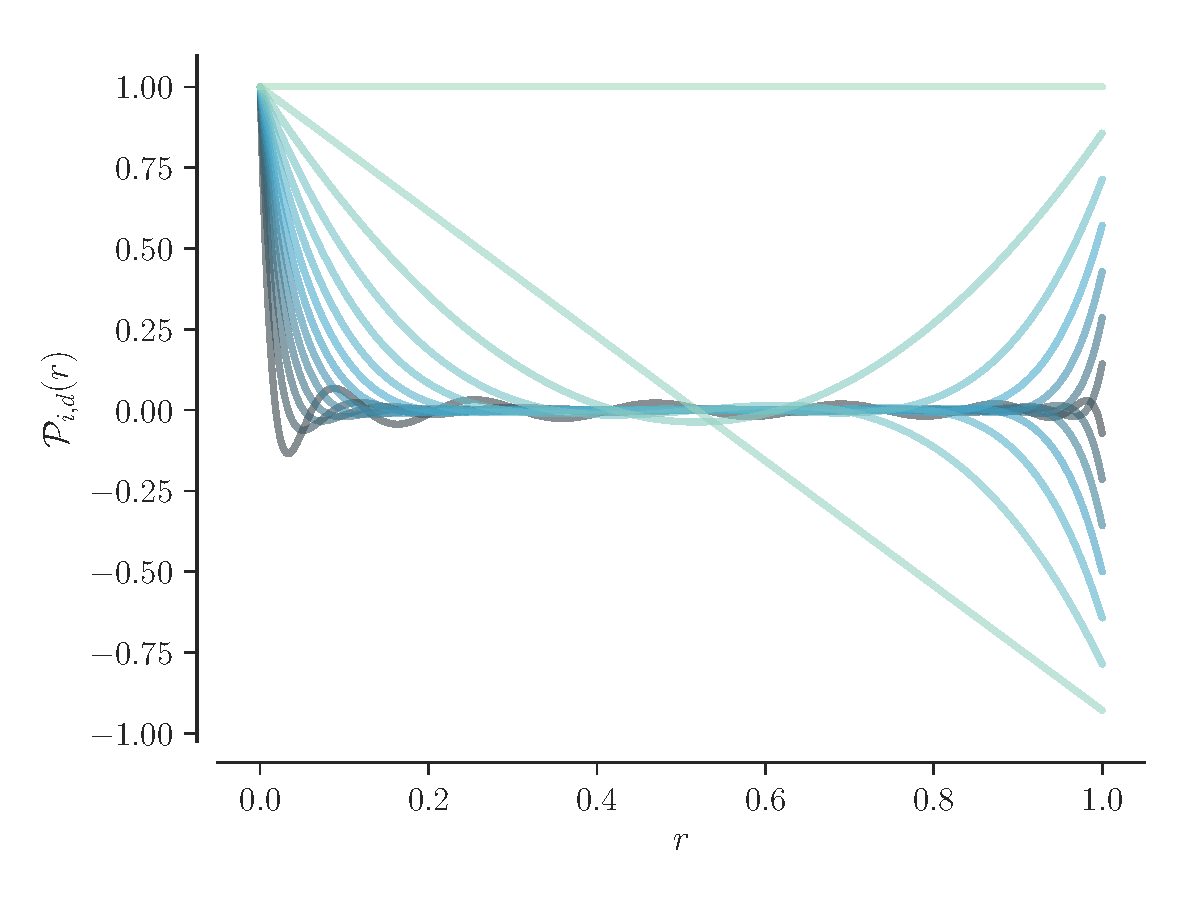
\includegraphics[width=\linewidth]{basis.pdf}
  \caption{ \label{fig:basis}
    Polynomial basis functions $\mathcal{P}_{i, d}$ from (\ref{eq:basis-functions}) with $d = 14$.
    Functions are sorted from $i = 0 \ldots d - 1$ by darkness.
    The state of the delay network, $\vec{x}(t)$, represents the rolling time window of input history by a linear combination of these functions (see~(\ref{eq:basis-interpretation})).
  } 
\end{minipage}\hfill
\begin{minipage}[b]{.32\textwidth}
  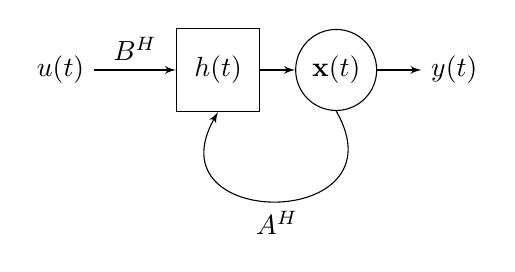
\begin{tikzpicture}[auto, >=latex']
    \node [input] (u) {$u(t)$};
    \node [block, right of=u, node distance=2cm] (h) {$h(t)$};
    \node [ensemble, right of=h, node distance=1.5cm] (x) {$\vec{x}(t)$};
    \node [output, right of=x, node distance=1.5cm] (y) {$y(t)$};
    \draw [->] (u) -- node {$B^H$} (h);
    \draw [->] (h) -- (x);
    %\draw [->] (x.north) -- (y);
    \draw [->] (x) -- (y);
    %\draw [->] (x.south) -- (y);
    \path[->] (x.south) edge [loop below, min distance=5em, out=-60, in=-120] node {$A^H$} (h.south);
  \end{tikzpicture}
  \caption{ \label{fig:architecture}
    Delay network~(DN) architecture.
    The synapse model $h(t)$ is driven by $A^H \vec{x}(t) + B^H u(t)$ to yield the state $\vec{x}(t)$. 
    This state is nonlinearly encoded by a heterogeneous population of neurons and subsequently decoded to estimate the desired $y(t)$.
  } 
\end{minipage}\hfill
\begin{minipage}[b]{.32\textwidth}
  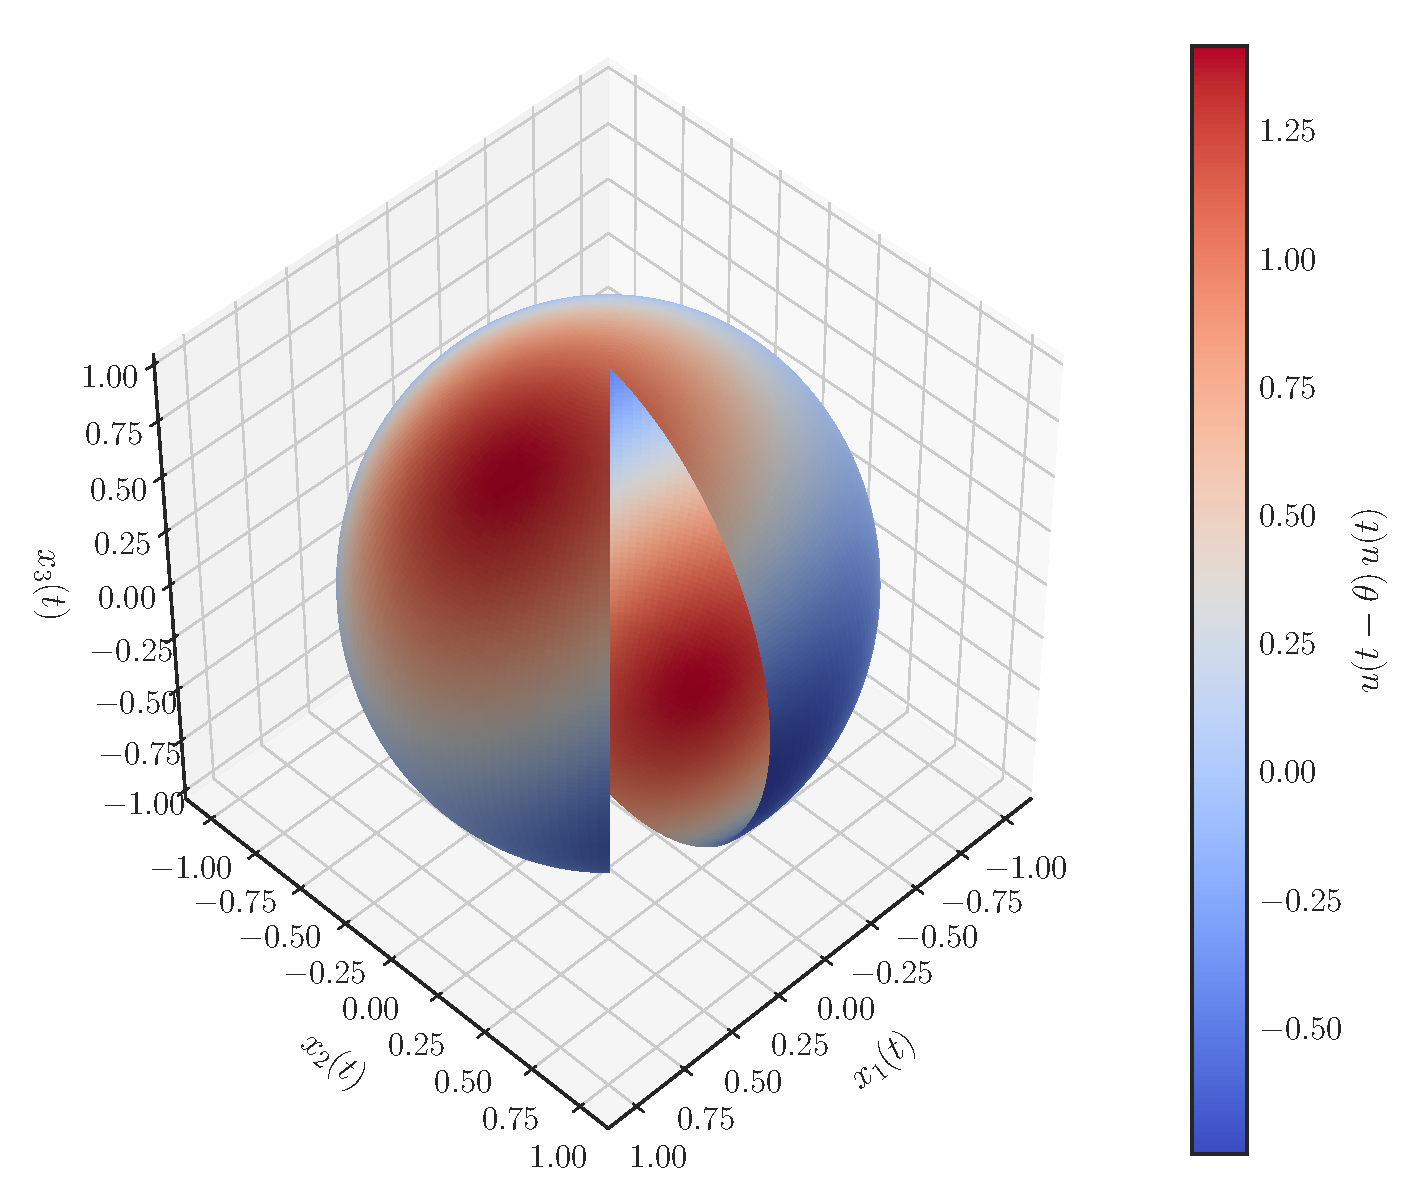
\includegraphics[width=\linewidth]{autocorrelation.pdf}
  \caption{ \label{fig:autocorrelation} 
    Visualizing the autocorrelation function $y(t) = u(t - \theta)\, u(t)$ with $d=3$.
    Each point along the surface of the unit-sphere is $\vec{x}(t)$, and is colored according to its corresponding value of $y(t)$ obtained from (\ref{eq:basis-interpretation}).
    A slice of the shell is cut away for visualization.
  } 
\end{minipage}
\end{figure*}

To implement this system as a recurrent neural network, we use the Neural Engineering Framework~\citep[NEF;][]{eliasmith2003neural} to map (\ref{eq:delay-system}) onto the dynamics of a lowpass synapse with time-constant $\tau$:
\begin{equation}
A^H = \tau A + I \text{,} \quad B^H = \tau B \text{,} \quad H(s) = \left(\tau s + 1\right)^{-1} \text{.}
\end{equation}
The resulting ``delay network''~(DN) is depicted in Figure~\ref{fig:architecture}.
Generalizations to arbitrary linear synapses, including those modelling pure feedback delays, may be found in %\cite{voelker2017b}.
\cite{voelkerdelay2017}.
The state $\vec{x}(t)$ is \emph{encoded} by a heterogeneous population of neurons, which allows arbitrary nonlinear functions across the window, $y(t) = f(\vec{x}(t))$, to be \emph{decoded} from its activity~\citep{eliasmith2003neural}.

We use Nengo~2.5~\citep{bekolay2014} and nengolib~0.4 %~\citep{nengolib},
to construct each network.
To demonstrate our ability to compute nonlinear window functions, we consider the function $y(t) = u(t - \theta)\, u(t)$, visualized in Figure~\ref{fig:autocorrelation}.
When integrated over time, this is the autocorrelation of $u$ with lag $\theta$, which has numerous applications in signal processing (e.g.,~detecting repeating events).
We fix $\theta = 0.1$\,s across all experiments.
To compute this function accurately, we sample a proportion of the encoders from the diagonal combinations of $\mathcal{P}_{i, d}(0)$ and $\mathcal{P}_{i, d}(1)$.
The inputs $u(t)$ are drawn from white-noise, band-limited with a cut-off frequency of $30$\,Hz.
Nengo allows us to consider populations of either spiking LIF neurons or non-spiking sigmoid neurons, without any additional changes to the model specification.
To optimize for the decoders, we map $d$-dimensional evaluation points onto desired target outputs using (\ref{eq:basis-interpretation}), and apply Nengo's regularized least squares solver, which avoids the need to explicitly simulate the network on any input signals.

To compare with Reservoir Computing, we ported a Python implementation of the Echo State Network~(ESN), from \cite{lukovsevivcius2009reservoir}, to Nengo, and implemented it analogously to the DN.
We used Hyperopt~\citep{bergstra2015hyperopt} to explore the space of model hyperparameters (e.g.,~$d$, $\tau$, input gain, recurrent gain, L2-regularization) across $100$ iterations containing $10$ trials each.
Each network consisted of $1\text{,}000$ neurons, simulated with a time-step of $1$\,ms.
Each trial used a training signal of length $10\text{,}200$, a testing signal of length $2\text{,}200$, and the first $200$ outputs were discarded.
We then cross-validated the best set of hyperparameters (in terms of mean normalized RMSE across all test signals) using another $25$ trials.
Complete source code may be found at \url{https://github.com/arvoelke/cosyne2018}.

We obtained a mean normalized RMSE of $0.059$ for the sigmoid DN, and $0.518$ for the spiking DN, compared to $0.843$ for the ESN.
Reducing the input frequency to $15$\,Hz improves the ESN's accuracy to be on par with the non-spiking DN, and thus we attribute this difference to the inherent difficulty of autocorrelating a high-frequency signal (relative to $\theta$) using random feedback weights, as opposed to using optimally derived weights as in the DN.
In addition, trials took on average $5.10$\,s for the sigmoid DN, $6.44$\,s for the spiking DN, and $17.7$\,s for the ESN.
This difference is a consequence of not simulating the DN for training, and from using factorized weight matrices (i.e.,~encoders and decoders) to simulate the DN.

\iffalse
We map this system onto the dynamics of a linear synapse $H(s) = \left( \sum_{i=0}^k c_i s^i \right)^{-1}$, via a generalization of NEF's Principle~3 (see Figure~?):
\begin{equation} \label{eq:general-linear}
\begin{aligned}
A^H &= \sum_{i=0}^k c_i A^i \text{,} & \quad B^H &= \left( \sum_{j=0}^{k-1} s^j \sum_{i=j+1}^k c_i A^{i-j-1} \right) B \text{,} %C^H &= C \text{,} \quad D^H &= D \text{,}
\end{aligned}
\end{equation}
For instance, the canonical lowpass synapse model $H(s) = \left( \tau s + 1 \right)^{-1}$ yields the standard form of Principle 3: $A^H = \tau A + I$, $B^H = \tau B$~\citep{eliasmith2003neural}.
\fi

\begin{multicols}{2}
\bibliographystyle{apacite}
\bibliography{abstract}
\end{multicols}

\end{document}